\documentclass{article}
\usepackage[utf8]{inputenc}
\usepackage{graphicx}

\title{nuclear}
\author{jenni }
\date{February 2016}

\begin{document}

\maketitle

\section{Introduction}
Nuclear half life tell us how long it takes for Nuclear processes to occur, so nuclear processes is where number protons and neutrons an atom's nucleus with a number of those protons and neutrons. Half life is the time that it takes for one hap a certain amount to decay to turn into protactinium to disappear(not real disappear, it becomes to the other thing). Half life that time required for half of a sample to decay.

\section{Experiment nuclear}
The initial number of atoms:10000
The probability of decay:0.5

\begin{figure}[h!]
\centering
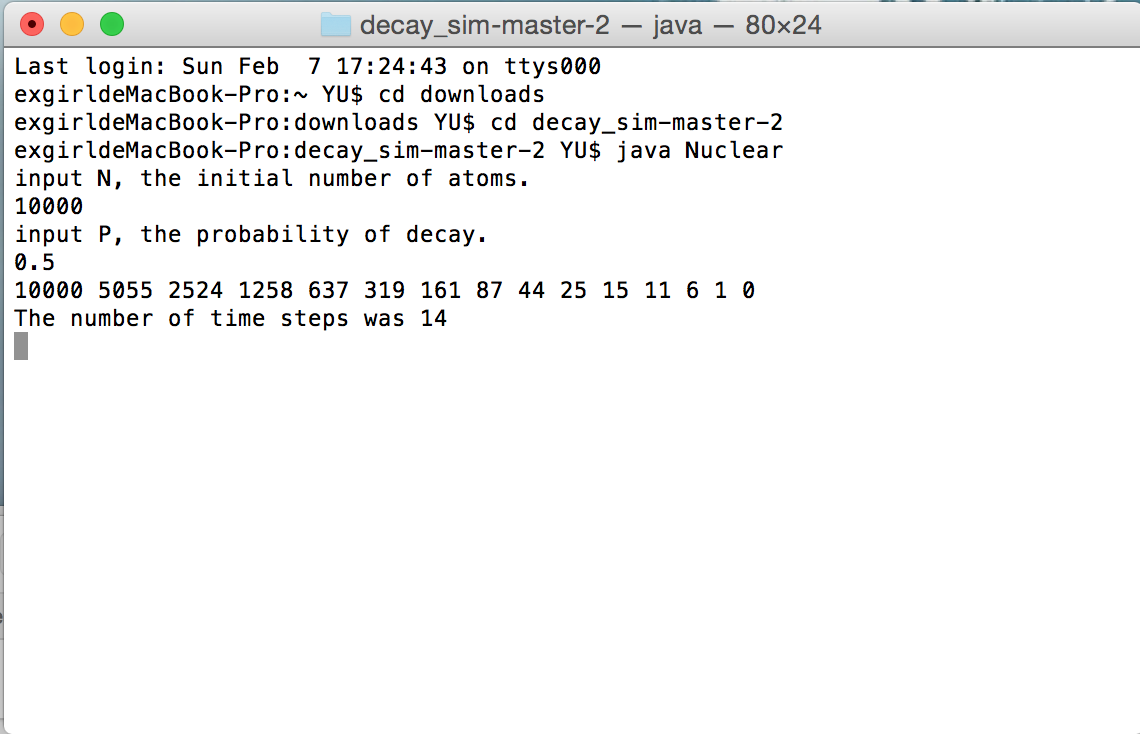
\includegraphics{1.png}
\caption{Nuclear}
\label{fig:nuclear}
\end{figure}

\begin{figure}[h!]
\centering
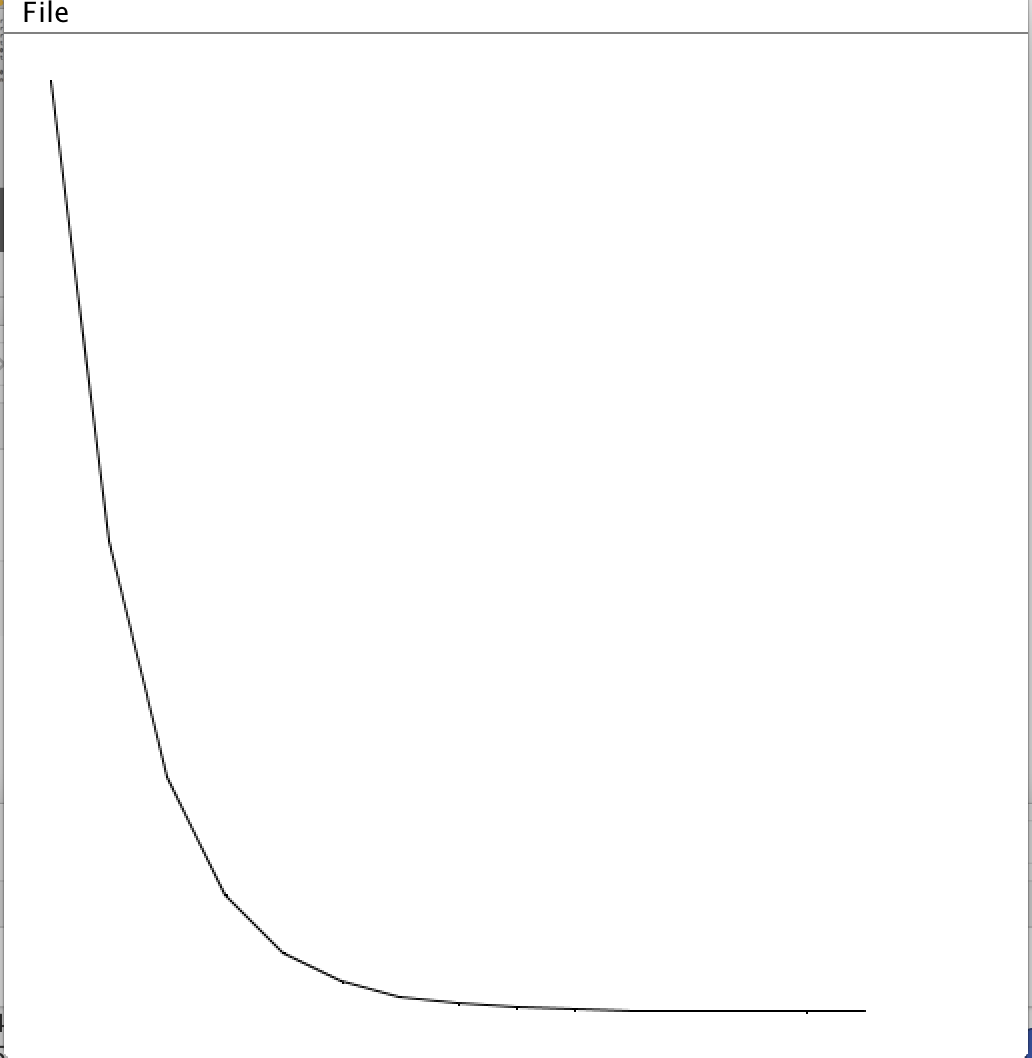
\includegraphics{2.png}
\caption{Nuclear}
\label{fig:nuclear}
\end{figure}


\begin{figure}[h!]
\centering
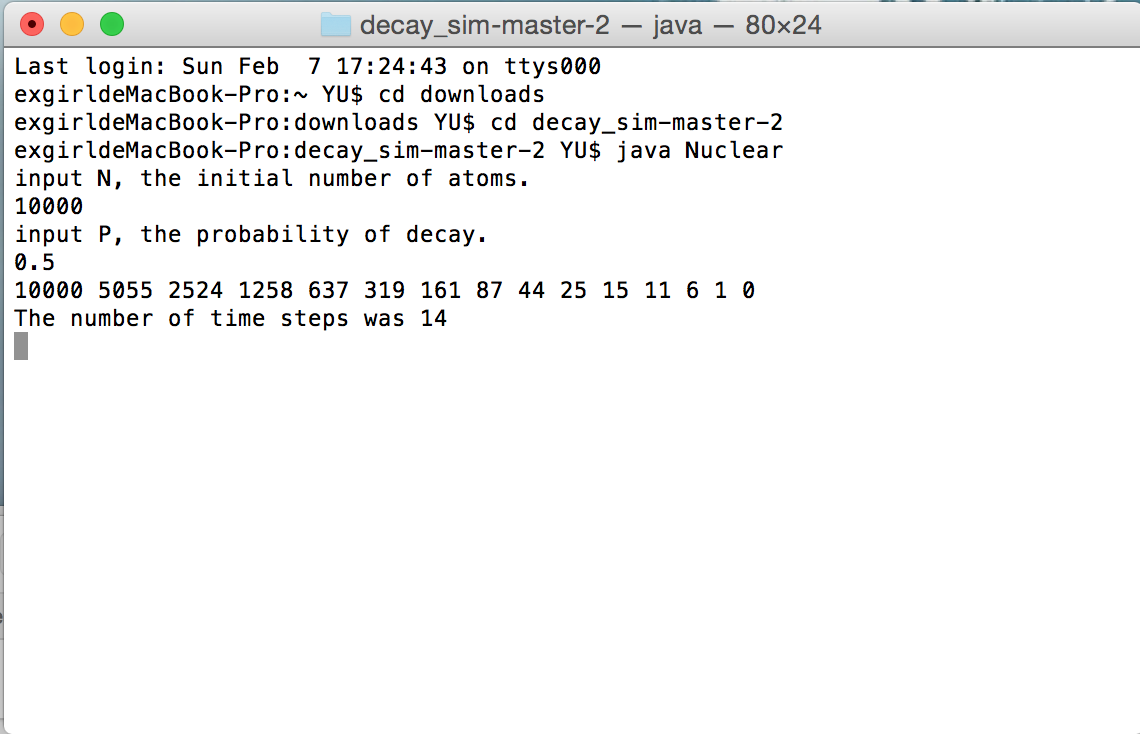
\includegraphics{4.png}
\caption{Nuclear}
\label{fig:nuclear}
\end{figure}

\begin{figure}[h!]
\centering
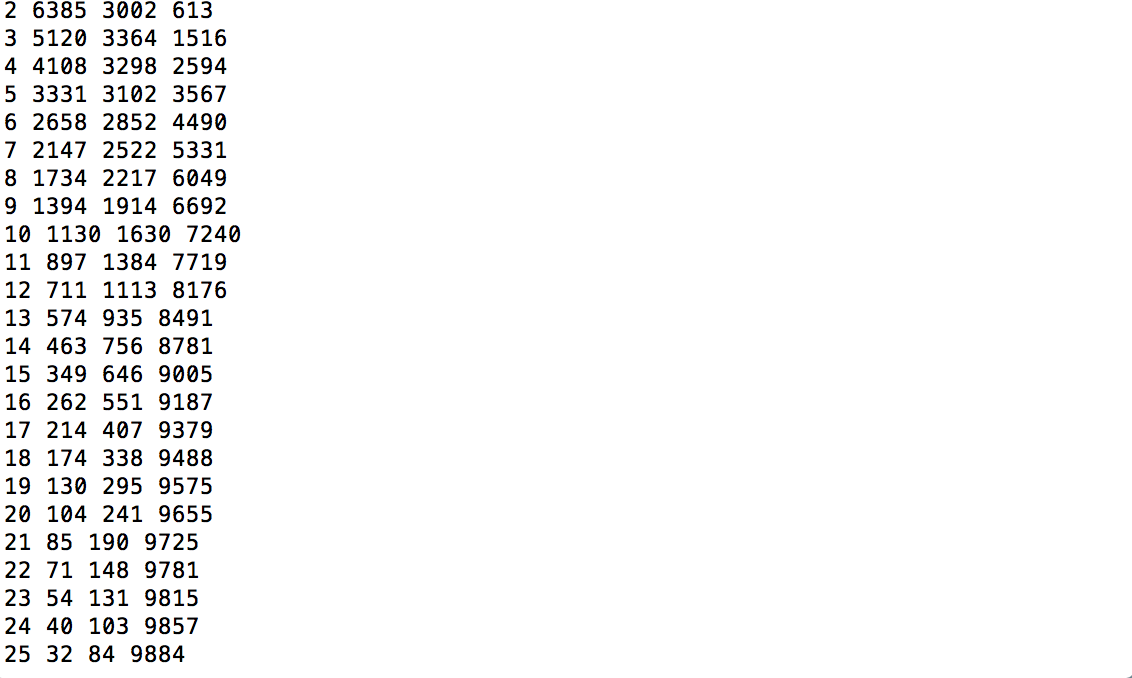
\includegraphics{5.png}
\caption{Nuclear}
\label{fig:nuclear}
\end{figure}

\begin{figure}[h!]
\centering
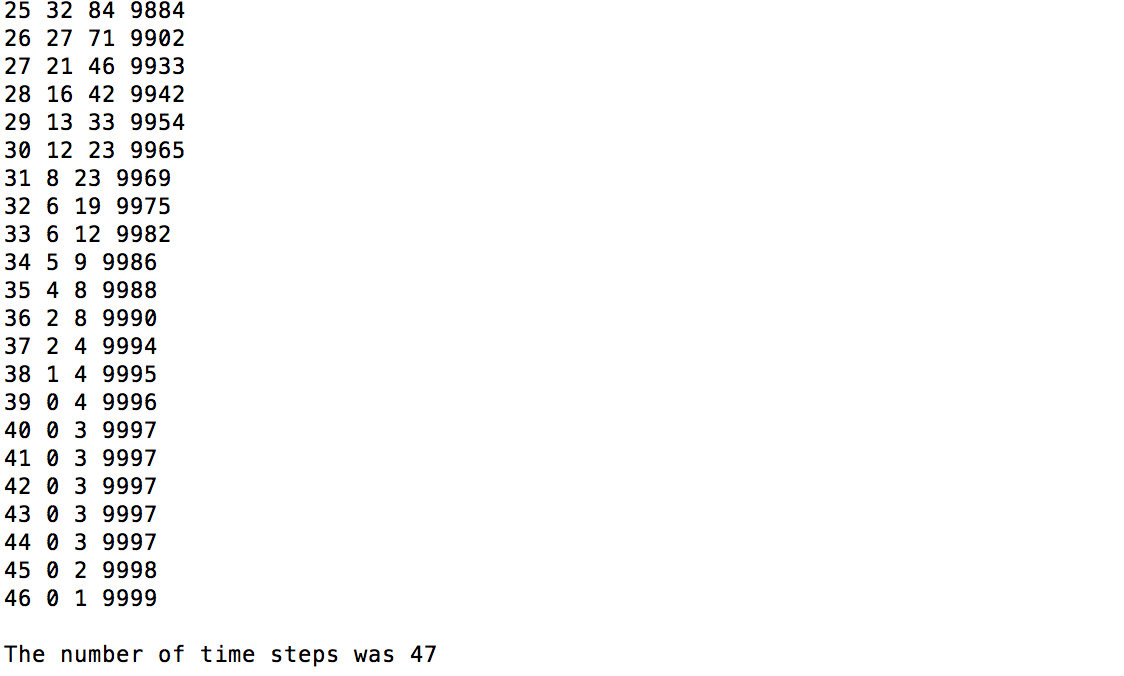
\includegraphics{6.png}
\caption{Nuclear}
\label{fig:nuclear}
\end{figure}



\begin{figure}[h!]
\centering
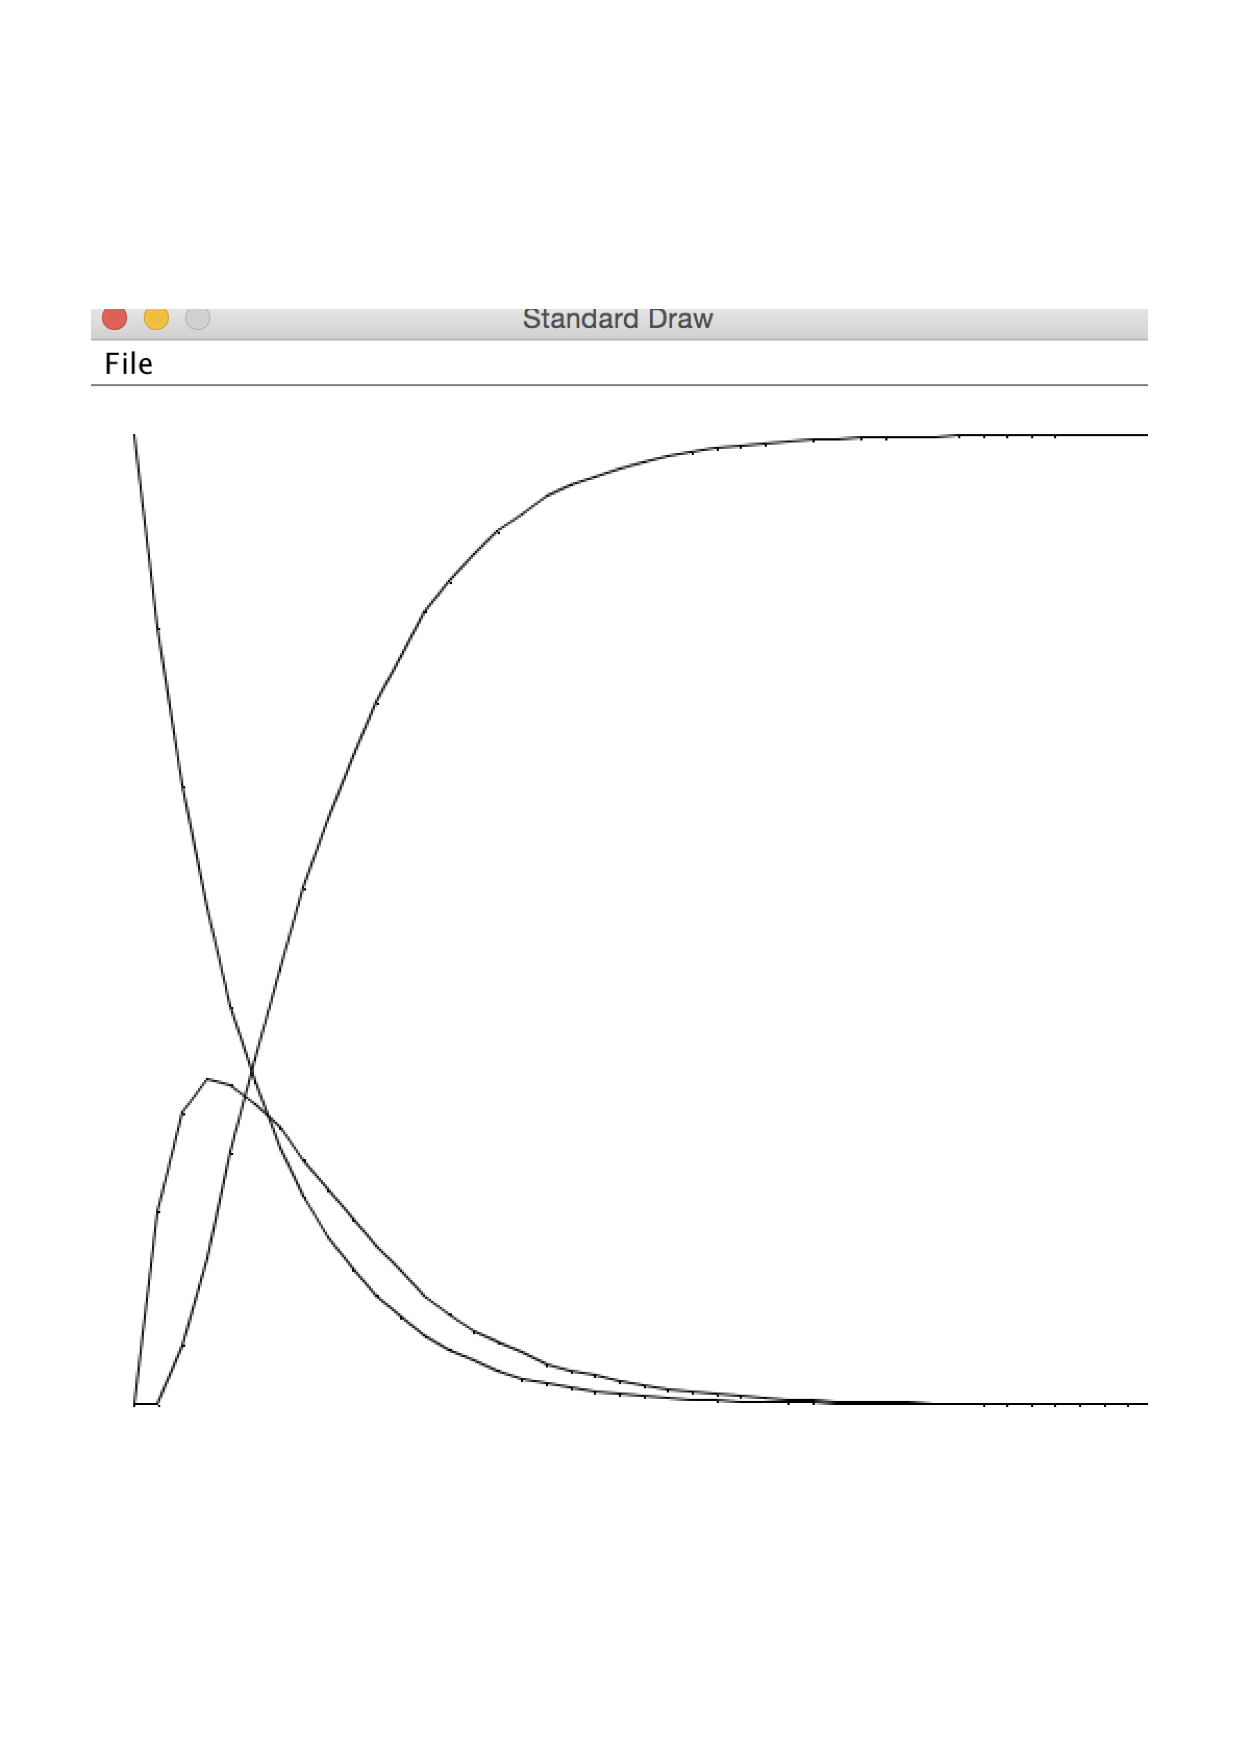
\includegraphics{7.png}
\caption{Nuclear}
\label{fig:nuclear}
\end{figure}



\end{document}
